\begin{enumerate}[\bfseries \mbox{Problema} 1.]

    %-------------------- problema 1
    \item Sean \textbf{\boldmath $x,y \in \mathbb{R}$ con $x,y\neq 0$. Si $\|x\|=\|y\|,$ entonces hallar la medida del ángulo entre $\frac{1}{2}(x+y)$ e $y-x$.\\\\
	Respuesta.-}\; Ya que $x,y\neq 0$ y por el teorema de los cosenos se tiene,
	\begin{equation}
	\left\langle \frac{1}{2}(x+y),y-x \right\rangle = \|x\|\|y\|\cos \theta 
	\end{equation}
	Por definición de producto interno y la parte izquierda de $(1)$,
	$$\sum_{i=1}^n \left[\dfrac{1}{2}(x_i+y_i)\cdot (y_i-x_i) \right]= -\dfrac{1}{2}\left(\sum_{i=1}^n x_i^2+\sum_{i=1}^n y_i^2\right) = -\dfrac{1}{2}\left(\langle x,x\rangle + \langle y,y\rangle \right).$$

	Así $(1)$ quedará de la siguiente manera,
	$$\langle x,x\rangle + \langle y,y\rangle = -2\|x\|\|y\|\cos \theta.$$

	Ya que $\|x\|=\|y\|$ y el teorema de cosenos. Entonces,
	$$\|x\|\|x\|\cos \theta + \|y\|\|y|\cos \theta = -2\|x\|\|x\|\cos \theta \quad \Rightarrow \quad \cos \theta \left(3\|x\|\|x\|+\|y\|\|y|\right)=0$$
	Por lo tanto,
	$$\cos \theta = 0 \quad \Rightarrow \quad \theta = \arccos(0) \quad \Rightarrow \quad \theta = \dfrac{\pi}{2}.$$\\
	

    %-------------------- problema 2
    \item \textbf{\boldmath Demuestre que si $x+y$ y $x-y$ son ortogonales, entonces los vectores $x$ e $y$ deben tener la misma longitud.\\\\
	Demostración.-}\; Sea $x.y\in \mathbb{R}^n$. Por definición de ortogonalidad, se tiene
	$$\langle x+y,x-y \rangle=0.$$
	Luego por definición de producto interno,
	$$\begin{array}{rcl}
	    \displaystyle\sum_{i=1}^n \left[(x_i+y_i)(x_i-y_i) \right]&=&0\\\\
	    \displaystyle\sum_{i=1}^n x_i^2 - \displaystyle\sum_{i=1}^n y_i^2&=&0\\\\
	    \langle x,x\rangle - \langle y,y\rangle &=&0\\\\
	    \sqrt{\langle x,x\rangle}&=&\sqrt{\langle y,y\rangle}\\\\
				     \|x\|&=&\|y\|\\
	\end{array}$$
	Ya que la norma mide el tamaño del vector entonces $x$ e $y$  tienen la misma longitud.\\\\


    %-------------------- problema 3
    \item \textbf{\boldmath Sean $x,y\in \mathbb{R}^n$. Demuestre que $\|x+y\|^2=\|x\|^2+\|y\|^2$ si, y solamente si, $x$ e $y$ son ortogonales.\\\\
	Demostración.-}\; Sea $\|x+y\|^2=\|x\|^2+2\langle x,y\rangle + \|y\|^2$. Como $\langle x,y\rangle = 0$, entonces
	$$\|x+y\|^2=\|x\|^2 + \|y\|^2.$$\\


    %-------------------- problema 4
    \item \textbf{\boldmath Demuestre, y dé una interpretación geométrica de, la ley del paralelogramo: Si $x,y\in \mathbb{R}^3$, entonces:
	$$\|x+y\|^2 + \|x-y\|^2=2\left(\|x\|^2+\|y\|^2\right).$$\\
    Demostración.-}\; Ya que $x,y\in \mathbb{R}^3$ y por definición de norma, entonces
    $$\begin{array}{rcl}
	\|x+y\|^2 + \|x-y\|^2 &=& \left(\sqrt{\langle x+y,x+y\rangle}\right)^2+\left(\sqrt{\langle x-y,x-y\rangle}\right)^2\\\\
			      &=&\displaystyle\sum_{i=1}^3 \left[(x_i+y_i)(x_i+y_i)\right]+\sum_{i=1}^3 \left[(x_i-y_i)(x_i-y_i)\right]\\\\
			      &=&\displaystyle\sum_{i=1}^3\left(x_i^2+2x_iy_i+y_i^2\right)+\displaystyle\sum_{i=1}^3\left(x_i^2-2x_iy_i+y_i^2\right)\\\\
			      &=&\displaystyle 2\left(\sum_{i=1}^3x_i^2+\sum_{i=1}^3y_i^2\right) = 2\left(\langle x,x\rangle+\langle y,y\rangle\right)\\\\
			      &=& 2\left[\left(\sqrt{\langle x,x\rangle}\right)^2+\left(\sqrt{\langle y,y\rangle}\right)^2\right]\\\\
			      &=& 2\left(\|x\|^2+\|y\|^2\right).\\\\
    \end{array}$$
    Otra manera de demostrar sería:
    $$\|x+y\|^2 + \|x-y\|^2 = \|x\|^2 + 2\langle x,y\rangle + \|y\|^2 + \|x\|^2 - 2\langle x,y\rangle + \|y\|^2 = 2\left(\|x\|^2+\|y\|^2 \right).$$\\


    %-------------------- problema 5
    \item \textbf{\boldmath Calcule el ángulo formado por los diagonales de dos caras consecutivas de un cubo de arista igual a $a$.\\\\
	Demostración.-}\; Ya que se tiene un cubo. Entonces,\\
	\begin{center}
	    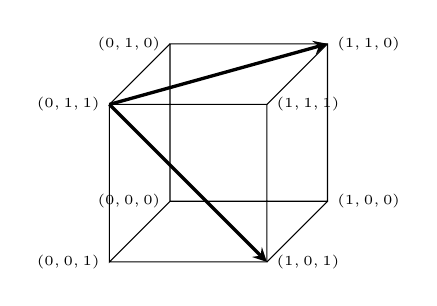
\begin{tikzpicture}[scale=2]
		\draw[](0,0,0)node[left]{\tiny$(0,0,0)$}--(0,1,0)node[left]{\tiny$(0,1,0)$}--(1,1,0)node[right]{\tiny$(1,1,0)$}--(1,0,0)node[right]{\tiny$(1,0,0)$}--(0,0,0)--(0,0,1)node[left]{\tiny$(0,0,1)$}--(0,1,1)node[left]{\tiny$(0,1,1)$}--(1,1,1)node[right]{\tiny$(1,1,1)$}--(1,0,1)node[right]{\tiny$(1,0,1)$}--(0,0,1);
		\draw[](1,1,1)--(1,1,0);
		\draw[](0,1,1)--(0,1,0);
		\draw[](1,0,1)--(1,0,0);
		\draw[line width=1.2pt,-stealth](0,1,1)--(1,0,1);
		\draw[line width=1.2pt,-stealth](0,1,1)--(1,1,0);
	    \end{tikzpicture}
    \end{center}
    Luego se tiene los vectores $$x=(1,0,1)-(0,1,1)=(1,-1,0) \quad \mbox{e} \quad y = (1,1,0)-(0,1,1)=(1,0,-1).$$ 
    Así, el ángulo $\theta$ estará dado por,
    $$\begin{array}{rcl}
	\cos \theta &=& \dfrac{\langle (1,-1,0),(1,0,-1)\rangle}{\|(1,-1,0)\|\|(1,0,-1)\|}\\\\ 
		    &=& \dfrac{1\cdot 1 + (-1)\cdot 0 + 0\cdot (-1)}{\sqrt{1^2+(-1)^2+0^2}\cdot \sqrt{1^2+0^2+(-1)^2}}\\\\
		    &=&\dfrac{1}{\left(\sqrt{2}\right)^2}=\dfrac{1}{2}.\\\\
    \end{array}$$
    Por lo tanto,
    $$\theta = \dfrac{\pi}{3}$$\\

    %-------------------- problema 6
    \item \textbf{\boldmath Demuestre que todo triángulo inscrito en una semicircunferencia es recto.\\\\
	Demostración.-}\; Representamos la idea con la siguiente gráfica.
	\begin{center}
	    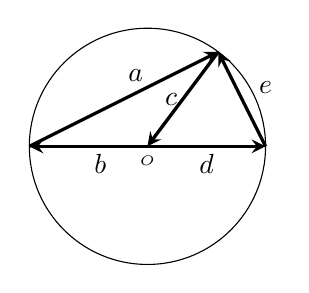
\begin{tikzpicture}[scale=1.5]
		\draw(0,0)circle(1);
		\draw[line width=1.2pt,stealth-](-1,0)--(0,0);
		\draw[line width=1.2pt,-stealth](0,0)--(1,0);
		\draw[line width=1.2pt,-stealth](-1,0)--(.6,.8);
		\draw[line width=1.2pt,-stealth](1,0)--(.6,.8);
		\draw[line width=1.2pt,-stealth](.6,.8)--(0,0);
		\draw(-0.1,.6)node[]{$a$};
		\draw(-.4,-.15)node[]{$b$};
		\draw(.2,.4)node[]{$c$};
		\draw(.5,-.15)node[]{$d$};
		\draw(1,.5)node[]{$e$};
		\draw(0,0)node[below]{\tiny$O$};
	    \end{tikzpicture}
	\end{center}
	Donde $a,b,c,d,e\in \mathbb{R}^n$ y $O$ el centro de la circunferencia, por lo tanto los vectores $b,d,c$ son iguales e inscritos en una semicircunferencia. Debemos demostrar que $\langle a,e\rangle=0$.\\ 

	Sean
	$$a=c+b, \quad  e=c+d \quad \mbox{y}\quad \|b\|=\|c\|=\|d\|$$

	Entonces por las propiedades de producto interno tenemos,
	$$\langle a,e\rangle = \langle c+b,c+d\rangle =\langle c+b, c\rangle + \langle c+b, d\rangle = \langle c,c \rangle +\langle c,b\rangle +\langle c,d\rangle +\langle b,d \rangle.$$

    	Ya que $\langle x,x \rangle = \|x\|^2\;$ y $\; b=-d$, nos queda:

	$$\langle a,e\rangle = \|c\|^2 -\langle c,d\rangle +\langle c,d\rangle -\|d\|^2 = 0.$$\\


    %-------------------- problema 7
    \item \textbf{\boldmath Demuestre que uniendo los puntos medios de los lados de un cuadrilátero se obtiene un paralelogramo.\\\\
	Demostración.-}\;

    %-------------------- problema 8
    \item \textbf{\boldmath Demuestre que el punto medio de la hipotenusa de un triángulo rectángulo es equidistante de los tres vertices.\\\\
	Demostración.-}\;

    %-------------------- problema 9
    \item \textbf{\boldmath Demuestre que el segmento que une los puntos medios de dos lados de un triángulo es paralelo al tercer lado y tiene la mitad de su longitud.\\\\
	Demostración.-}\; Consideremos el siguiente gráfico. Sean $a,b,c,d\in \mathbb{R}^n$ 
	\begin{center}
	    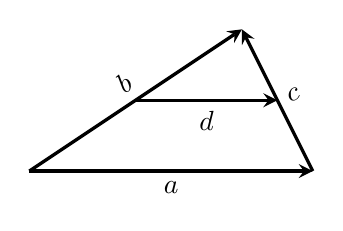
\begin{tikzpicture}[scale=.9]
		\draw[line width=1.2pt,-stealth](0,0)--(4,0) node[rotate=0,pos=0.5, below]{$a$};
		\draw[line width=1.2pt,-stealth](0,0)--(3,2) node[rotate=35,pos=0.5, above]{$b$};
		\draw[line width=1.2pt,-stealth](4,0)--(3,2) node[rotate=20,pos=0.5, right]{$c$};
		\draw[line width=1.2pt,-stealth](1.5,1)--(3.5,1) node[rotate=0,pos=0.5, below]{$d$};
	    \end{tikzpicture}
	\end{center}
	de donde podemos deducir las siguientes ecuaciones:

	$$\left\{\begin{array}{rcl}
		\dfrac{b}{2}-\dfrac{c}{2}-d&=&0\\\\
		a+\dfrac{c}{2}-d-\dfrac{b}{2}&=&0\\
	\end{array}\right. \quad \Rightarrow \quad 
	\left\{\begin{array}{rcl}
		\dfrac{c}{2}&=&\dfrac{b}{2}-a\\\\
		\dfrac{c}{2}&=&d+\dfrac{b}{2}-a\\\\
	\end{array}\right.$$

	Entonces $a=2d$ si y sólo si $a \parallel d$. Así tomando la norma nos queda:
	$$\|a\|=\|2d\| \quad \Rightarrow \quad \|d\|=\dfrac{1}{2}\|a\|.$$\\

    %-------------------- problema 10
    \item \textbf{\boldmath Pruebe la ley de senos utilizando vectores.\\\\
	Demostración.-}\; Considere el siguiente triangulo.
	\begin{center}
	    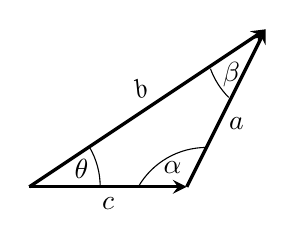
\begin{tikzpicture}[scale=1]
		\draw[line width=1.2pt,-stealth](0,0)--(2,0) node[rotate=0,pos=0.5, below]{$c$};
		\draw[line width=1.2pt,-stealth](2,0)--(3,2) node[rotate=0,pos=0.4, right]{$a$};
		\draw[line width=1.2pt,-stealth](0,0)--(3,2) node[rotate=20,pos=0.5, above]{$b$};
		\draw(.9,0) arc (0:30:1)node[pos=.43,left]{$\theta$};
	        \draw(2.25,.5) arc (90:150:1)node[pos=.7,right]{$\alpha$};
	        \draw(2.3,1.5) arc (200:225:1)node[pos=.2,right]{$\beta$};
	    \end{tikzpicture}
	\end{center}
	Sea $a,b,c \in \mathbb{R}^3$. Notemos que $b=c+a$ por lo que utilizaremos la proposición $$\|x \times y\| = \|x\|\|y\| \sen(\theta)$$
	de la siguiente manera. Sea $x\times x = 0$ de donde,
	\begin{itemize}

	    \item $\sen(\theta) = \dfrac{\|b\times c\|}{\|b\|\|c\|}=\dfrac{\|(c+a)\times c|\|}{\|b\|\|c\|}=\dfrac{\|c\times c + a\times c\|}{\|b\|\|c\|}=\dfrac{\|a\times c\|}{\|b\|\|c\|}.$ Entonces,
		$$\dfrac{\sen(\theta)}{\|a\|}=\dfrac{\|a\times c\|}{\|a\|\|b\|\|c\|}$$

	    \item $\sen(\alpha) = \dfrac{\|c\times a\|}{\|a\|\|c\|}=\dfrac{\|(b-a)\times a|\|}{\|a\|\|c\|}=\dfrac{\|a\times b - a\times a\|}{\|a\|\|c\|}=\dfrac{\|a\times b\|}{\|a\|\|c\|}.$ Entonces,
		$$\dfrac{\sen(\alpha)}{\|b\|}=\dfrac{\|a\times c\|}{\|a\|\|b\|\|c\|}$$

	    \item $\sen(\beta) = \dfrac{\|b\times a\|}{\|a\|\|b\|}=\dfrac{\|(c+a)\times a|\|}{\|a\|\|b\|}=\dfrac{\|c\times a - a\times a\|}{\|a\|\|b\|}=\dfrac{\|a\times c\|}{\|a\|\|b\|}.$ Entonces,
		$$\dfrac{\sen(\beta)}{\|c\|}=\dfrac{\|a\times c\|}{\|a\|\|b\|\|c\|}$$

	\end{itemize}
	Por lo tanto,
	$$\dfrac{\sen(\theta)}{\|a\|}=\dfrac{\sen(\alpha)}{\|b\|}=\dfrac{\sen(\beta)}{\|c\|}.$$\\



    %-------------------- problema 11
    \item \textbf{\boldmath Muestre que las medianas de un triángulo se cortan en un punto a un tercio de cada mediana.\\\\
	Demostración.-}\;

    %-------------------- problema 12
    \item \textbf{\boldmath Demuestre que las diagonales de un rombo son ortogonales entre si.\\\\
	Demostración.-}\; Sean $a,b,c,d,e,f\in \mathbb{R}^n.$ De donde gráficamente se tiene:
	\begin{center}
	    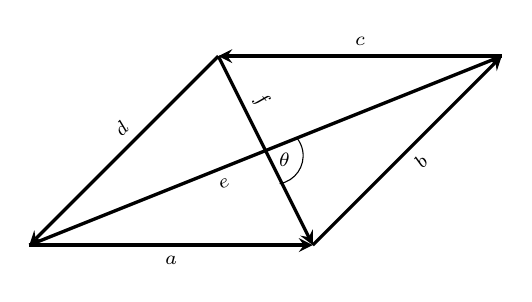
\begin{tikzpicture}[scale=1.2]
	      \tikzstyle{every node}=[font=\scriptsize]
	      \draw[line width=1.2pt,-stealth](0,0)--(3,0) node[rotate=0,pos=0.5,below]{$a$};
	      \draw[line width=1.2pt,-stealth](3,0)--(5,2) node[rotate=50,pos=0.5, below]{$b$};
	      \draw[line width=1.2pt,-stealth](5,2)--(2,2) node[rotate=0,pos=0.5, above]{$c$};
	      \draw[line width=1.2pt,-stealth](2,2)--(0,0) node[rotate=45,pos=0.45, above]{$d$};
	      \draw[line width=1.2pt,-stealth](0,0)--(5,2) node[rotate=23,pos=0.4, below]{$e$};
	      \draw[line width=1.2pt,-stealth](2,2)--(3,0) node[rotate=-50,pos=0.3, above]{$f$};
	      \draw(2.65,.65) arc (-80:40:.3);
	      \draw(2.7,.9)node[]{$\theta$};
	    \end{tikzpicture}
	\end{center}
	Así,  $$\cos (\theta) = \dfrac{\langle e,f\rangle}{\|e\|\|f\|} \quad \Rightarrow \quad \theta = \cos^{-1}\left(\dfrac{\langle a+b, d+a\rangle}{\|e\|\|f\|}\right).$$

	Luego, ya que $a,b,c,d$ forman un rombo. Es decir, un paralelogramo de lados iguales, entonces $d=-b$, por lo que:
	$$\theta = \cos^{-1}\left(\dfrac{\langle a+b, -b+a\rangle}{\|e\|\|f\|}\right).$$
	Por las propiedades de producto interno y $\|a\|=\|b\|$,
	$$\begin{array}{rcl}
	    \theta&=&\cos^{-1}\left(\dfrac{\langle a,-b\rangle+\langle b,-b\rangle+\langle a,a\rangle+\langle b,a\rangle}{\|e\|\|f\|}\right)\\\\
		  &=&\cos^{-1}\left(\dfrac{-\langle a,b\rangle-\langle b,b\rangle+\langle a,a\rangle+\langle a,b\rangle}{\|e\|\|f\|}\right)\\\\
		  &=&\cos^{-1}\left(\dfrac{\langle a,a\rangle-\langle b,b\rangle}{\|e\|\|f\|}\right)\\\\
		  &=&\cos^{-1}\left(\dfrac{\|a\|^2-\|b\|^2}{\|e\|\|f\|}\right)\\\\
		  &=& \cos^{-1}\left(\dfrac{0}{\|e\|\|f\|}\right) = \dfrac{\pi}{2}.\\\\
	\end{array}$$
	Por lo tanto,
	$$e\perp f.$$\\


    %-------------------- problema 13
    \item \textbf{\boldmath Si $x,y,z \in \mathbb{R}^3,$ entonces demostrar que:
	$$x\times (y \times z) = \langle x,z\rangle y - \langle x,y\rangle z.$$\\
	Demostración.-}\; Calculemos $y\times z$.
	$$y\times z = \left|\begin{array}{ccc}
	    e_1 & e_2 & e_3 \\
	    y_1 & y_2 & y_3 \\
	    z_1 & z_2 & z_3
	\end{array}\right| = \left(y_2z_3-y_3z_2,y_3z_1-y_1z_3, y_1z_2-y_2z_1\right)$$

	Luego, calculemos $x\times (y \times z)$

	$$\begin{array}{rcl}
	    x\times (y\times z) &=& \left|\begin{array}{ccc}
	    e_1 & e_2 & e_3 \\
	    x_1 & x_2 & x_3 \\
	    y_2z_3-y_3z_2 & y_3z_1-y_1z_3 & y_1z_2-y_2z_1
	\end{array}\right|\\\\
	&=& \left[x_2\left(y_1z_2-y_2z_1\right)-x_3\left(y_3z_1-y_1z_3\right)\; , \; x_3\left(y_2z_3-y_3z_2\right)-x_1\left(y_1z_2-y_2z_1\right),\right.\\
	&&\left.x_1\left(y_3z_1-y_1z_3\right)-x_2\left(y_2z_3-y_3z_2\right)\right]\\\\
	&=& \left(x_2y_1z_2-x_2y_2z_1-x_3y_3z_1+x_3y_1z_3\; , \; x_3y_2z_3-x_3y_3z_2-x_1y_1z_2+x_1y_2z_1\right.\\
	&&\left.x_1y_3z_1-x_1y_1z_3-x_2y_2z_3+x_2y_3z_2\right).\qquad (1)\\\\
	\end{array}$$

	Por otro lado calculamos $\langle x,z\rangle y - \langle x,y\rangle z$.

	$$\begin{array}{rcl}
	    &&(x_1z_1+x_2z_2+x_3z_3)(y_1,y_2,y_3)-(x_1y_1+x_2y_2+x_3y_3)(z_1,z_2,z_3)\\\\
	    &=& (x_1y_1z_1+x_2y_1z_2+x_3y_1z_3\; ,\; x_1y_2z_1+x_2y_2z_2+x_3y_2z_3\; , \; x_1y_3z_1+x_2y_3z_2+x_3y_3z_3)\\
	    &-&(x_1y_1z_1+x_2y_2z_1+x_3y_3z_1\; , \; x_1y_1z_2+x_2y_2z_2+x_3y_3z_2\; ,\; x_1y_1z_3+x_2y_2z_3+x_3y_3z_3)\\\\
	    &=&(x_2y_1z_2+x_3y_1z_3-x_2y_2z_1-x_3y_3z_1\; , \; x_1y_2z_2+x_3y_2z_3-x_1y_1z_2-x_3y_3z_2 ,\\
	    &=& x_1y_3z_1+x_2y_3z_2-x_1y_1z_3-x_2y_2z_3). \qquad (2)\\\\
	\end{array}$$
	Igualando (1) y (2) concluimos que,
	$$x\times (y \times z) = \langle x,z\rangle y - \langle x,y\rangle z.$$\\

    %-------------------- problema 14
    \item \textbf{\boldmath Sean $x,y\in \mathbb{R}^3$ con $x,y\neq 0.$ Si $\dfrac{\|x\times y\|}{\|x\|^3}=3,$ entonces hallar $\dfrac{\| \langle x,x\rangle y - \langle x,y\rangle x \|}{\|x\|^4}$.\\\\
	Respuesta.-}\;

    %-------------------- problema 15
    \item \textbf{\boldmath Si $x,y\in \mathbb{R}^3$, entonces demostrar que:
    $$\|x\times y\|^2 = \|x\|^2 \|y\|^2 - \langle x,y \rangle^2.$$\\
	Demostración.-}\;
	Dado que $\langle x,y\rangle =\|a\|\|b\|\cos \theta,$ entonces
	$$\|x\|^2\|y\|^2-\langle x, y\rangle^2=\|x\|^2\|y\|^2-\|x\|^2\|y\|^2\cos^2\theta = \|x\|^2\|y\|^2\left(1-\cos^2 \theta\right).$$
	Ya que $1-\cos^2\theta = \sen^2\theta$, se sigue
	$$\|x\|^2\|y\|^2-\langle x, y\rangle^2=\left(\|x\|\|y\|\sen \theta\right)^2$$
	Luego por el hecho de que $\|x\times y\|=\|x\|\|y\|\sen \theta$, nos queda:
	$$\|x\|^2\|y\|^2-\langle x, y\rangle^2=\|x\times y\|^2.$$\\
	


    %-------------------- problema 16
    \item \textbf{\boldmath Si $x,y,z \in \mathbb{R}^3,$ entonces demostrar que:
    $$x\times (y\times z) + y \times (z\times x)+z\times(x\times y)=0.$$\\
	Demostración.-}\; Por el problema 13, sabemos que $x\times (y \times z) = \langle x,z\rangle y - \langle x,y\rangle z$. Por lo tanto,
	$$x\times (y\times z) + y \times (z\times x)+z\times(x\times y) = \langle x,z\rangle y- \langle x,y\rangle z + \langle y,x\rangle z -\langle y,z \rangle x +\langle z,y\rangle x -\langle z,x\rangle y.$$

	Luego, por la propiedad de conmutatividad concluimos que:

	$$\langle x,z\rangle y- \langle x,y\rangle z + \langle x,y\rangle z -\langle y,z \rangle x +\langle y,z\rangle x -\langle x,z\rangle y = 0.$$\\

\end{enumerate}
